% What the First Stage Cannot Detect --- AER: Insights short version
% Compiles with pdflatex. No title page: title and byline sit at the top of page 1.
\documentclass[11pt]{article}

\usepackage[margin=1in]{geometry}
\usepackage{amsmath,amssymb,amsthm}
\usepackage{booktabs}
\usepackage{pgfplots}
\pgfplotsset{compat=1.18}
\usepgfplotslibrary{groupplots,fillbetween}
\usepackage{setspace}
\usepackage[hidelinks]{hyperref}
\usepackage{natbib}
\bibliographystyle{aer}

\setstretch{1.15}
\setlength{\emergencystretch}{2em}

\theoremstyle{plain}
\newtheorem{lemma}{Lemma}
\newtheorem{proposition}{Proposition}
\newtheorem{corollary}{Corollary}
\theoremstyle{definition}
\newtheorem{assumption}{Assumption}

\newcommand{\E}{\mathbb{E}}
\newcommand{\Cov}{\operatorname{Cov}}
\newcommand{\Var}{\operatorname{Var}}
\newcommand{\Lb}{\bar{L}}
\newcommand{\Zt}{\tilde{Z}}
\newcommand{\bx}{b(X)}
\newcommand{\indep}{\perp\!\!\!\perp}

\begin{document}

% ---- Title and byline at the top of the first page (no title page) ----
\renewcommand{\thefootnote}{\fnsymbol{footnote}}
\begin{center}
{\Large\bfseries What the IV First Stage Cannot Detect}\\[6pt]
{\large Parush Arora\footnote{Department of Economics, Ashoka University. Email: \texttt{parush.arora@ashoka.edu.in}.}}
\end{center}
\renewcommand{\thefootnote}{\arabic{footnote}}
\setcounter{footnote}{0}

\vspace{2.5em}

\begin{abstract}
\noindent Applied instrumental-variable practice reads a large first-stage $F$, increasingly the conditional $F$ of \citet{sw2016}, as a license to interpret the second-stage estimate, and it is not one. In just-identified linear IV with a binary instrument, a binary treatment, and covariates entered linearly, an exact decomposition writes the 2SLS bias as a covariance between the curvature of the instrument propensity and the covariate level functions. That same object builds the first-stage covariance the conditional $F$ is computed from, so a single nuisance both biases the estimand and inflates the reported strength. The contamination then acts in two distinct failure modes. In the first, under instrument--covariate collinearity, the curvature inflates the $F$ while the identifying signal vanishes. In the second, even with an honest and enormous $F$, the bias hides entirely on the outcome side. We prove that within this class no first-stage diagnostic is informative about the bias. This covers the conditional $F$, the effective $F$ of \citet{mop2013}, and the Cragg--Donald statistic, indeed any functional of the law of $(Z,D,X)$. The bias is pinned down only by the conditional law of the outcome. A directed conditional-moment test, built from reduced-form regressions alone and valid even under weak identification, has power exactly where the $F$ is silent. In the canonical 401(k) design a conditional $F$ above 7{,}000 conceals a wealth effect understated by about a third, which the test flags and the correction repairs.\\[4pt]
\noindent\textit{JEL}: C26, C21, C52. \quad \textit{Keywords}: instrumental variables, LATE, first-stage strength, contamination bias, specification testing.
\end{abstract}

\clearpage

\section{Introduction}

In the canonical study of 401(k) saving, eligibility instruments participation with a conditional first-stage $F$ above seven thousand, four orders of magnitude past any weak-instrument threshold. The design looks beyond reproach, yet it is biased. With income entered linearly, which is the standard specification, the estimated effect of participation on net financial assets is understated by about a third, and no statistic computed from the instrument and the treatment reveals it. Strength and bias are objects of different stages of the model, and this paper shows exactly when and why they come apart. The claim is confined to a specific setting that we mark throughout, namely a binary instrument, a binary treatment, just identification, and covariates entered linearly.

The instrumental-variable estimator is the workhorse of applied microeconomics whenever treatment is suspected to be endogenous. Its credibility rests on two pillars. The first is the exclusion restriction, defended by argument and sensitivity analysis. The second is the strength of the first stage, treated as a statistical object to be certified. A large literature has produced size-based procedures for diagnosing weak instruments \citep{staigerstock1997,stockyogo2005,mop2013,assw2019}, and reporting a first-stage $F$ is now routine, indeed mandatory in most journals. When the model contains covariates, \citet{sw2016} show that the relevant object is the \emph{conditional} first-stage $F$, computed after partialling the covariates out of the instrument, and applied work increasingly reports it.

Running in parallel, a second literature has clarified \emph{what} a strong instrument identifies under treatment-effect heterogeneity. Since \citet{imbensangrist1994} it has been understood that IV recovers a local average treatment effect (LATE), the effect on compliers. Most consequential for practice is \citet{blandhol2022}. Once covariates enter the second stage \emph{linearly}, the near-universal specification, 2SLS is in general \emph{not} a convex-weighted average of LATEs unless the covariates are entered nonparametrically (``saturated''). \citet{gpi2024} give a general treatment of the contamination that additive adjustment induces across \emph{multiple} treatments, and \citet{zhao2025} establish that linearity of the instrument propensity $\E[Z\mid X]$ in the covariates is necessary and sufficient for a LATE interpretation.

These two literatures leave open the question a practitioner actually faces. Does the strength diagnostic tell you anything about this? The strength literature certifies that the instrument moves the treatment. The heterogeneity literature characterizes what the movement identifies. The implicit bridge in applied work, that a strong conditional first stage licenses a causal reading of the second stage, has never been examined. We show it is false, and, more sharply, that \emph{no} first-stage diagnostic can repair it. A second question is whether checking the propensity is enough, and it is not. A propensity-only check such as a RESET on $\E[Z\mid X]$ cannot distinguish a biased design from an unbiased one with equally nonlinear propensity, because whether the nonlinearity matters depends on the outcome. In independent, concurrent work, \citet{krummewestphal2026} develop a test of IV validity that accommodates flexible covariate specifications. They show that it also detects the bias induced by covariate misspecification, and they reach the related conclusion that such a diagnostic must be directed at the outcome rather than at the propensity alone.\footnote{Their procedure tests a joint null of instrument validity and correct covariate specification through density-based bounds on the always- and never-taker outcome means, and requires a first stage strong enough to estimate the complier share. Ours conditions on validity, isolates the contamination in a single reduced-form conditional-moment restriction, and stays size-controlled under weak identification.}

The starting point is an exact Frisch--Waugh--Lovell (FWL) decomposition of the just-identified 2SLS estimand. Writing $e(x)=\E[Z\mid X=x]$ for the instrument propensity, $h(x)$ for the component of $e(x)$ orthogonal to the linear covariate span (the ``propensity curvature''), $p(x)$ for the conditional first stage, and $m_D,m_Y$ for the covariate level functions,
\begin{equation}\label{eq:decomp-intro}
\beta_{2SLS}=\frac{\overbrace{\E[e(X)\{1-e(X)\}p(X)\,\mathrm{LATE}(X)]}^{\text{signal }S_Y}+\overbrace{\Cov(h(X),m_Y(X))}^{\text{contamination }\theta_Y}}{\underbrace{\E[e(X)\{1-e(X)\}p(X)]}_{\text{signal }S_D}+\underbrace{\Cov(h(X),m_D(X))}_{\text{contamination }\theta_D}}.
\end{equation}
The signal ratio $S_Y/S_D\equiv\Lb$ is the convex-weighted average of conditional LATEs of \citet{blandhol2022}. Each contamination term is a covariance that vanishes exactly when the propensity curvature is orthogonal to the relevant level function. The subject of this paper is a feature of \eqref{eq:decomp-intro} that has gone unremarked. The \emph{denominator} $S_D+\theta_D$ is exactly the first-stage covariance the conditional $F$ is built from, so the same nuisance $\theta_D$ that biases the estimand also inflates the reported strength.

Because the contamination sits in both the numerator and the denominator, it produces two distinct failure modes. In \emph{mode~(a)}, manufactured strength, the instrument is nearly collinear with the covariates. The denominator contamination dominates, the identifying signal $S_D$ vanishes, and the conditional $F$ is inflated by the very curvature that biases the estimand. In \emph{mode~(b)}, invisible outcome-side bias, the strength is honest. Now $\theta_D$ and the contamination share are small and the $F$ is genuinely large, yet the estimand is biased through the numerator term $\theta_Y$, which loads on the outcome, where no first-stage number can see it. The two modes share one root cause. Strength is a first-stage object, while the bias is an outcome object. We characterize the collinearity limit (Proposition~\ref{prop:collim}), show the conditional $F$ diverges rather than collapses along it, and prove that \emph{no} first-stage functional can detect the bias (Proposition~\ref{prop:imposs}). We then construct a directed test that uses the outcome, show it is size-controlled under weak identification (Proposition~\ref{prop:weakid}), and apply it to a panel of canonical designs. The flagship 401(k) design turns out to be a clean instance of mode~(b).

\section{The strength--bias identity and the impossibility result}\label{sec:framework}

Let $Z\in\{0,1\}$ be a binary instrument, $D\in\{0,1\}$ a binary treatment, $Y\in\mathbb{R}$ an outcome, and $X\in\mathbb{R}^{d_x}$ covariates, with potential treatments $D(z)$ and potential outcomes $Y(d)$. We maintain the standard conditional-on-$X$ LATE assumptions. (i) Conditional validity, $\{Y(d),D(z)\}\indep Z\mid X$ and exclusion. (ii) Conditional monotonicity, $D_i(1)\ge D_i(0)$ a.s. (iii) Conditional relevance, $p(x)\equiv\E[D\mid Z=1,X=x]-\E[D\mid Z=0,X=x]>0$ on a set of positive probability with overlap $0<e(x)<1$, which makes $S_D=\E[e(X)\{1-e(X)\}p(X)]>0$ and the benchmark $\Lb=S_Y/S_D$ well defined. The analyst estimates the just-identified linear IV model $Y=\beta D+X'\gamma+\varepsilon$ with $Z$ the single excluded instrument and $(1,X')$ included, so that with $\Zt\equiv Z-L(Z\mid 1,X)$ the linear projection residual, $\beta_{2SLS}=\E[\Zt Y]/\E[\Zt D]$.

Define the propensity $e(x)=\E[Z\mid X=x]$, its linear projection $\ell(x)=L(Z\mid 1,X)(x)$, and the propensity curvature $h(x)\equiv e(x)-\ell(x)$, which satisfies $\E[h(X)]=0$ and $\E[h(X)r(X)]=0$ for every affine $r$. Let $m_D(x)=\E[D\mid X=x]$, $m_Y(x)=\E[Y\mid X=x]$, and $\mathrm{LATE}(x)=\E[Y(1)-Y(0)\mid D(1)>D(0),X=x]$.

\begin{lemma}[Contamination decomposition]\label{lem:decomp}
Under the maintained assumptions,
\[
\beta_{2SLS}=\frac{S_Y+\theta_Y}{S_D+\theta_D},\qquad
\beta_{2SLS}-\Lb=\frac{\theta_Y-\Lb\,\theta_D}{S_D+\theta_D},\qquad S_D+\theta_D=\E[\Zt D],
\]
where
\[
\begin{aligned}
&S_Y=\E[e(X)\{1-e(X)\}p(X)\mathrm{LATE}(X)], && S_D=\E[e(X)\{1-e(X)\}p(X)],\\
&\theta_Y=\Cov(h(X),m_Y(X))=\E[h(X)Y], && \theta_D=\Cov(h(X),m_D(X))=\E[h(X)D].
\end{aligned}
\]
\end{lemma}

\noindent The identity comes from splitting the residualized instrument as $\Zt=(Z-e(X))+h(X)$. The experimental part $Z-e(X)$ carries the complier signal, giving $S_D$ for $D$ and, through the conditional Wald identity, $S_Y$ for $Y$. The projection error $h(X)$ is orthogonal to affine functions, so it contributes only the level-function covariances $\theta_D$ and $\theta_Y$. Appendix~\ref{app:proofs} gives the proof, and \citet{arora2026} the extended results.

The signal ratio $\Lb=S_Y/S_D$ is a proper, non-negatively weighted average of conditional LATEs. The contamination terms are covariances between the nonlinear part of the propensity and the nonlinear part of the level functions. A linear propensity ($h\equiv 0$) kills both and reproduces \citet{blandhol2022}, while linearity of a single level function kills only its own term.

The decomposition has one unremarked feature that organizes the paper. The denominator of the 2SLS estimand equals the population first-stage covariance $\E[\Zt D]=S_D+\theta_D$ from which the \citet{sw2016} conditional $F$ is built, and the contamination $\theta_D$ is the common term. It enters the bias $\beta_{2SLS}-\Lb=(\theta_Y-\Lb\theta_D)/(S_D+\theta_D)$ and, being a signed covariance, inflates the reported first-stage covariance when $\theta_D>0$. Strength and interpretability can be driven by the same nuisance. Through the denominator the contamination inflates the reported strength (mode~a). Through the numerator, via $\theta_Y$, it biases the estimand even when the reported strength is honest (mode~b). We now show that no first-stage diagnostic can detect either.

We first formalize collinearity, where ``$Z$ is collinear with $X$'' means $\Var(Z\mid X)=e(X)\{1-e(X)\}$ is small. Index a sequence of data-generating processes by $t$ along which four conditions hold. (i) $e_t(x)\{1-e_t(x)\}\to 0$ a.e.\ and $\E[e_t(X)\{1-e_t(X)\}]\to 0$. (ii) The curvature converges, $h_t\to h^\ast$ in $L^2$ with $h^\ast$ nondegenerate. (iii) $\mathrm{LATE}_t,p_t,m_{D,t},m_{Y,t}$ converge in $L^2$. (iv) $\Cov(h^\ast,m_D^\ast)\neq 0$, a genericity condition ruling out knife-edge cancellation.

\begin{proposition}[Collinearity limit]\label{prop:collim}
Along such a sequence the signal terms vanish, $S_{D,t}\to 0$ and $S_{Y,t}\to 0$, while the contamination terms converge to $\Cov(h^\ast,m_D^\ast)\neq 0$ and $\Cov(h^\ast,m_Y^\ast)$. Hence
\[
\beta_{2SLS,t}\longrightarrow \frac{\Cov(h^\ast,m_Y^\ast)}{\Cov(h^\ast,m_D^\ast)},
\]
a ratio of covariate-level contrasts with no LATE interpretation, which may lie outside the range of the conditional LATEs $\mathrm{LATE}^\ast(\cdot)$ and even take the opposite sign of every $\mathrm{LATE}^\ast(x)$.
\end{proposition}

The reduced-form intuition is transparent. As $\Var(Z\mid X)\to 0$ the within-covariate-cell experimental variation disappears. All that survives in $\Zt$ is the projection error $h(X)$, a deterministic function of $X$, so the estimator compares $Y$ and $D$ across covariate cells with weights $h(X)$, exactly the comparison an IV design is meant to avoid. The payoff for practice is that the strength diagnostic does not warn.

The strength diagnostic itself shows the same divergence. The population \citet{sw2016} conditional first-stage slope is $\pi_t=\E[\Zt_t D]/\Var(\Zt_t)\to \Cov(h^\ast,m_D^\ast)/\E[(h^\ast)^2]\neq 0$. The conditional $F$, whose population counterpart is proportional to $n\,\pi_t^2\Var(\Zt_t)/\sigma_v^2$, is therefore bounded away from zero and \emph{diverges} with the sample size along the sequence, even though the estimand is pure contamination. A large conditional $F$ therefore places no bound on the bias. The conditional $F$ correctly certifies that $\Zt$ is a strong predictor of $D$. Under collinearity, however, $\Zt$ predicts $D$ through the contamination channel $h(X)$, not the complier variation $e(1-e)p$. The failure is not special to the conditional $F$.

\begin{proposition}[Strength diagnostics cannot detect contamination]\label{prop:imposs}
Let $T$ be any diagnostic that is a measurable functional of the joint distribution of $(Z,D,X)$, in particular any first-stage relevance or strength statistic, including the conditional $F$, the effective $F$ of \citet{mop2013}, and the Cragg--Donald statistic. Fix any such law with nonzero curvature, $h\neq 0$. Then $T$ is uninformative about the contamination bias. There exist data-generating processes with that common joint distribution of $(Z,D,X)$, hence identical values of $T$, but arbitrarily different biases $\beta_{2SLS}-\Lb$. Detecting the bias requires the conditional distribution of $Y$.
\end{proposition}

\noindent The intuition is that the bias depends on $\theta_Y=\E[h(X)Y]$ and on $\Lb=S_Y/S_D$, both functionals of the outcome that are left completely free once the law of $(Z,D,X)$ is fixed. Shifting the always- and never-taker outcome levels $\E[Y(d)\mid X]$ in the curvature direction $h$ changes $\theta_Y$, and hence the bias, while leaving $D=D(Z)$, the conditional LATEs, and the entire law of $(Z,D,X)$ unchanged, and with them every strength diagnostic. The gap can be made arbitrarily large, so $T$ carries no information about the bias. When $h\equiv 0$, Lemma~\ref{lem:decomp} already certifies $\theta_D=\theta_Y=0$, so the interesting case is exactly the one $T$ cannot resolve. Appendix~\ref{app:proofs} gives the construction.

A strength statistic summarizes how the instrument moves compliers, whereas the bias lives with the non-compliers, which is why strength cannot see it. A valid diagnostic must therefore use the outcome. One thing the first stage \emph{can} certify is the absence of curvature. By Lemma~\ref{lem:decomp}, $h\equiv 0$ forces $\theta_D=\theta_Y=0$, and $h$ is testable from $(Z,X)$ alone by a Ramsey RESET. But this cuts the wrong way for the applied bridge. RESET rejects for propensity curvature in \emph{any} direction, including curvature orthogonal to the outcome that leaves the bias untouched, so it cannot distinguish a biased design from an unbiased one with equally nonlinear propensity. The impossibility is conditional on nonzero curvature. Once $h\neq 0$, no first-stage functional can say whether that curvature is harmful, because harm runs through $\theta_Y$ and $\Lb$, which only the outcome pins down. This both motivates and disciplines the test of the next section, whose central moment $\theta_Y=\E[h(X)Y]$ is precisely such an outcome functional.

\section{A directed test and the cost of correction}\label{sec:test}

By Lemma~\ref{lem:decomp}, $\beta_{2SLS}=\Lb$ whenever $\theta_D=\theta_Y=0$. We test
\begin{equation}\label{eq:H0}
H_0:\ \theta_D=0\ \text{and}\ \theta_Y=0\qquad\text{against}\qquad H_1:\ (\theta_D,\theta_Y)\neq(0,0).
\end{equation}
Because $\theta_D=\E[h(X)D]$ and $\theta_Y=\E[h(X)Y]$ depend only on the propensity curvature and on observables, $H_0$ is a statement about the reduced form, and the consequential misspecification is nonlinearity of $\E[Z\mid X]$ in the directions that also load on $D$ and $Y$. This is what separates the test from a RESET, which fires for curvature in any direction. The directed statistic probes only curvature that loads on $D$ and $Y$, and does so without touching an endogenous regressor.

\paragraph{Estimator.} Let $\bx=(b_1(X),\dots,b_K(X))'$ be basis functions (polynomials or splines) orthogonalized against $(1,X')$ in the population, $\E[b(X)(1,X')]=0$. Model the propensity as $e(X)=\alpha_0+X'\alpha_1+b(X)'\delta+\rho(X)$ with $\E[\rho(X)b(X)]=0$, so the basis-captured curvature is $h_K(X)=b(X)'\delta$. Given an i.i.d.\ sample, the test is computed in three steps. First, regress $Z_i$ on $(1,X_i',b(X_i)')$ by OLS and form $\hat{h}_i=b(X_i)'\hat\delta$. Second, form the sample contamination moments $\hat\theta_D=n^{-1}\sum_i\hat h_i D_i$ and $\hat\theta_Y=n^{-1}\sum_i\hat h_i Y_i$, stacked as $\hat\theta=(\hat\theta_D,\hat\theta_Y)'$. Third, compute $W_n=n\,\hat\theta'\hat\Sigma^{-1}\hat\theta$, where $\hat\Sigma$ is consistent for the asymptotic variance $\Sigma$ of $\sqrt{n}\,\hat\theta$.

\begin{proposition}[Limiting distribution]\label{prop:limit}
Under standard two-step regularity with $K$ fixed, $\sqrt{n}(\hat\theta-\theta)\xrightarrow{d}N(0,\Sigma)$, where $\Sigma=\Var(\psi_i)$ and the influence function
\[
\psi_i=\begin{pmatrix}b(X_i)'\delta\,D_i-\theta_D\\ b(X_i)'\delta\,Y_i-\theta_Y\end{pmatrix}+\big(\E[Db(X)'],\ \E[Yb(X)']\big)'G^{-1}b(X_i)u_i
\]
carries the generated-regressor correction for first-stage estimation of $\delta$, with $G=\E[b(X)b(X)']$ and $u_i$ the first-stage residual. Under $H_0$, $W_n\xrightarrow{d}\chi^2_2$.
\end{proposition}

The test is consistent against any fixed alternative, since $W_n$ then diverges, and against local alternatives $\theta=\eta/\sqrt{n}$ it has noncentrality $\eta'\Sigma^{-1}\eta$. A nonparametric pairs bootstrap that recomputes $(\hat h,\hat\theta)$ on each resample is first-order valid and reproduces the generated-regressor term automatically. The decisive property is what the test does \emph{not} do. It never divides $\hat\theta$ by the first-stage covariance $\E[\Zt D]$.

\begin{proposition}[Size under weak identification, power under manufactured strength]\label{prop:weakid}
Along a weak-identification null sequence in which $S_{D,n}\to 0$ (as when $\Var(Z\mid X)\to 0$), the curvature stays nondegenerate ($h_n\to h^\ast\neq 0$), and $H_0$ holds, $W_n\xrightarrow{d}\chi^2_2$, so the test that rejects when $W_n>\chi^2_{2,1-\alpha}$ has asymptotic size $\alpha$ regardless of the degree of identification. Along the contaminated collinearity sequence of Proposition~\ref{prop:collim}, by contrast, $\theta_{D,n}\to\Cov(h^\ast,m_D^\ast)\neq 0$, the noncentrality diverges, and power tends to one, even as every first-stage strength diagnostic diverges.
\end{proposition}

The mechanism is that $\theta$ and $\psi$ are functionals of the reduced form $(Z,D,Y,X)$, estimated at rate $\sqrt{n}$ by the regression of $Z$ on $(1,X',b(X)')$, whose behavior is governed by $G=\E[bb']$ rather than by the relevance of the instrument. This is what separates the diagnostic from the natural saturate-and-compare alternative, which estimates $\beta$ under a saturated specification and forms a Hausman contrast against the linear estimate. Under collinearity that alternative is exactly the wrong tool, because saturating drives the effective instrument toward the vanishing signal $S_D\to 0$, so the saturated estimator is itself weakly identified and its sampling variability swamps the contrast. Our test sidesteps this because it never forms an IV ratio. When the propensity is estimated flexibly or by machine learning, a Neyman-orthogonalized moment $\psi^o_W(O;e,m_W)=h(X)W+\tilde m_W(X)(Z-e(X))-\theta_W$, with $\tilde m_W$ the level function detrended of its affine part, restores $\sqrt{n}$ inference under only $n^{1/4}$-consistent cross-fitted nuisances \citep{cchd+2018}.

\paragraph{A bias-targeting variant.} The null \eqref{eq:H0} is sufficient for $\beta_{2SLS}=\Lb$ but not necessary. The bias also vanishes under \emph{harmless curvature}, when $\theta_Y=\Lb\theta_D$ with $(\theta_D,\theta_Y)\neq(0,0)$, a nonlinear propensity whose curvature happens not to displace the estimand. The exact no-bias restriction is the single moment $H_0^\ast:\ \E[h(X)\{Y-\Lb D\}]=0$, necessary and sufficient for $\beta_{2SLS}=\Lb$. Testing $H_0^\ast$ requires plugging in $\Lb$ and is therefore pivotal only when $S_D$ is bounded away from zero, whereas the screening test \eqref{eq:H0} keeps its size exactly where $H_0^\ast$ loses pivotality. Because the two forms make opposite trade-offs between size and power across the collinearity range, the recommendation is to report both, the strongly identified screen \eqref{eq:H0} and, where identification is not in doubt, the bias-targeting confirmatory test.

\subsection{Bias-corrected estimation and the cost of correction}\label{sec:correct}

The decomposition suggests an immediate correction. Subtract the contamination from numerator and denominator. Since $\E[\Zt Y]-\theta_Y=\E[(Z-e(X))Y]$ and likewise for $D$, the corrected estimand equals the signal ratio $\Lb$. It is implemented by replacing the linear-projection residual $\Zt$ with the residual from a flexibly estimated propensity $\hat e(\cdot)$,
\begin{equation}\label{eq:corrected}
\hat\Lb=\frac{\sum_i\big(Z_i-\hat e(X_i)\big)Y_i}{\sum_i\big(Z_i-\hat e(X_i)\big)D_i}.
\end{equation}
This is the residualized-propensity, or partialling-out, IV estimator, and it coincides with the recommendation of \citet{blandhol2022} to saturate the covariates. It is consistent for $\Lb$ under only $L^2$-consistency of $\hat e$, with no orthogonality or rate condition, and asymptotic normality holds under standard conditions, though weak-instrument-robust confidence sets are appropriate when $S_D$ is small (Appendix~\ref{app:proofs}). Our contribution is not the estimator but the following statement of its cost, which the collinearity limit makes precise.

Beyond a hypothesis test, the decomposition yields a single interpretable number. Define the \emph{contamination share}
\begin{equation}\label{eq:share}
\varrho\equiv\frac{\theta_D}{S_D+\theta_D}=\frac{\theta_D}{\E[\Zt D]},
\end{equation}
the fraction of the observed first-stage covariance attributable to propensity curvature rather than to complier variation. It is estimated by $\hat\varrho=\hat\theta_D/\widehat{\E[\Zt D]}$ with a percentile-bootstrap interval and is meant to be read next to the conditional $F$. A large $F$ paired with a non-negligible $\hat\varrho$ signals that the strength is partly manufactured (mode~a). Crucially, $\varrho$ is a first-stage gauge and measures only mode~(a). It is \emph{not} a bias estimate, because by Proposition~\ref{prop:imposs} the bias also loads on the outcome-side term $\theta_Y$. A small $\hat\varrho$ therefore does not certify a design, as the 401(k) case of Section~\ref{sec:401k}, where $\hat\varrho=0.03$ yet the estimand is off by a third, will show.

But the correction is not free. The corrected estimator's own first-stage covariance is exactly the signal term $\E[(Z-e(X))D]=S_D$, which vanishes along the collinearity sequence of Proposition~\ref{prop:collim}. The corrected estimator is therefore weakly identified in precisely the regime in which the correction matters most. No specification of the covariates both removes the contamination and preserves the apparent first-stage strength, because the strength was the contamination. The trade-off is exact, since the corrected and reported first-stage covariances obey $S_D=(1-\varrho)\,\E[\Zt D]$, so the corrected concentration parameter carries a factor $(1-\varrho)^2$ and the fraction of identifying variation surrendered by correcting is the same $\varrho$ that measured how much of the apparent strength was contamination. A design with $\varrho\approx 0$, such as the 401(k) instrument below, is corrected at negligible cost, whereas a design whose strength is mostly curvature ($\varrho\to 1$) cannot be both corrected and strongly identified.

\section{Monte Carlo evidence}\label{sec:mc}

Throughout, $X\sim\text{Uniform}(-2,2)$ and $g(X)=X^2-\tfrac43$ (mean zero). Potential treatments satisfy monotonicity via a latent uniform, with conditional first stage $p(X)=0.4$, and the conditional LATE is heterogeneous and strictly positive, $\mathrm{LATE}(X)=1+0.25X\in[0.5,1.5]$. The outcome is $Y=A_\mu\,g(X)+\mathrm{LATE}(X)D+\mathcal{N}(0,1)$. A \emph{nonlinear} logit propensity $e(X)=\Lambda(\kappa\,g(X))$ indexes collinearity through $\kappa$, with larger $\kappa$ driving $\Var(Z\mid X)\to 0$. A \emph{linear-probability} propensity $e(X)=0.5+0.08X+b\,g(X)$ switches contamination off at $b=0$, where the propensity is affine and the null holds, so $b=0$ is exactly the no-contamination null.

\begin{table}[t]
\centering
\caption{Collinearity limit. 2SLS estimand versus the conditional $F$ ($n=200{,}000$, $A_\mu=1.5$, true $\mathrm{LATE}(X)\in[0.5,1.5]$). As $\kappa$ rises the estimand leaves the LATE hull and converges to the contamination limit $\Cov(h^\ast,m_Y^\ast)/\Cov(h^\ast,m_D^\ast)$, while the conditional $F$ stays four orders of magnitude above the threshold of 10.}
\label{tab:collim}
\begin{tabular}{rcccc}
\toprule
$\kappa$ & $\beta_{2SLS}$ & cond.\ $F$ & contam.\ limit & $\E[e(1-e)]$\\
\midrule
0.10 & 1.527 & 39{,}808 & 151.4 & 0.249\\
0.50 & 3.497 & 40{,}459 & 32.8 & 0.230\\
1.00 & 5.408 & 38{,}776 & 19.1 & 0.189\\
2.00 & 7.325 & 38{,}904 & 13.1 & 0.118\\
4.00 & 8.487 & 37{,}790 & 10.7 & 0.057\\
8.00 & 8.794 & 37{,}881 & 9.77 & 0.027\\
32.0 & 8.860 & 38{,}215 & 9.11 & 0.007\\
\bottomrule
\end{tabular}
\end{table}

Table~\ref{tab:collim} traces the nonlinear-propensity design as $\kappa$ rises, with $n=200{,}000$ to approximate the population. The 2SLS estimand leaves the LATE hull $[0.5,1.5]$ already at mild collinearity and converges monotonically to the theoretical contamination limit of Proposition~\ref{prop:collim}, while the conditional variance $\E[e(1-e)]$ collapses toward zero. Throughout, the conditional first-stage $F$ remains near 40{,}000, as the divergence result of Section~\ref{sec:framework} predicts. The strength diagnostic not only fails to warn, it grows more emphatic exactly as the estimand becomes pure contamination. Figure~\ref{fig:collim} plots the two panels.

\begin{figure}[t]
\centering
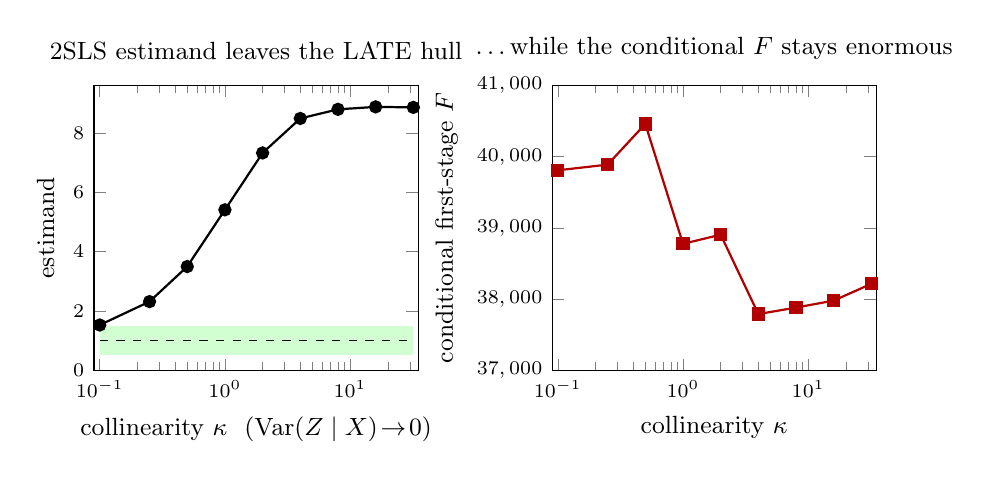
\begin{tikzpicture}
\begin{groupplot}[group style={group size=2 by 1, horizontal sep=1.7cm}, width=0.47\textwidth, height=5.2cm, xmode=log, log basis x=10, xmin=0.09, xmax=35, tick label style={font=\scriptsize}, label style={font=\small}, title style={font=\small}]
\nextgroupplot[xlabel={collinearity $\kappa$\ \ ($\Var(Z\mid X)\!\to\!0$)}, ylabel={estimand}, ymin=0, ymax=9.6, title={2SLS estimand leaves the LATE hull}]
\addplot[draw=none, name path=lo, forget plot] coordinates {(0.1,0.5) (32,0.5)};
\addplot[draw=none, name path=hi, forget plot] coordinates {(0.1,1.5) (32,1.5)};
\addplot[green!18, forget plot] fill between[of=lo and hi];
\addplot[black, dashed, forget plot] coordinates {(0.1,1.0) (32,1.0)};
\addplot[black, mark=*, thick] coordinates {(0.10,1.527) (0.25,2.316) (0.50,3.497) (1.00,5.408) (2.00,7.325) (4.00,8.487) (8.00,8.794) (16.0,8.877) (32.0,8.860)};
\nextgroupplot[xlabel={collinearity $\kappa$}, ylabel={conditional first-stage $F$}, ymin=37000, ymax=41000, scaled y ticks=false, yticklabel style={/pgf/number format/1000 sep={,}}, title={\dots while the conditional $F$ stays enormous}]
\addplot[red!70!black, mark=square*, thick] coordinates {(0.10,39808) (0.25,39888) (0.50,40459) (1.00,38776) (2.00,38904) (4.00,37790) (8.00,37881) (16.0,37979) (32.0,38215)};
\end{groupplot}
\end{tikzpicture}
\caption{As collinearity $\kappa$ rises (same design as Table~\ref{tab:collim}), the 2SLS estimand (left, solid) leaves the band of all conditional LATEs (shaded, $[0.5,1.5]$) and departs from the true convex-weighted LATE (dashed, $\approx 1$), converging to the contamination limit of Proposition~\ref{prop:collim}. Meanwhile the conditional first-stage $F$ (right) stays near $40{,}000$ throughout, four orders of magnitude above the weak-instrument threshold of 10.}
\label{fig:collim}
\end{figure}

Two exercises confirm the test's behavior. On a single large contaminated dataset ($n=100{,}000$, $\kappa=4$) the directed test rejects at $p<10^{-4}$ while the conditional $F$ is 20{,}723, and the bias-corrected estimator recovers the true convex-weighted LATE. Over 300 replications at $n=3{,}000$ the test has a conservative size of $1.3\%$ against the $5\%$ level under a linear propensity and power essentially one under a curved one, at a mean conditional $F$ near 575 in \emph{both} cases. The $F$ cannot discriminate the two designs that the test separates almost perfectly.

\subsection{Separating harmful from harmless curvature}

The directed test must do two things at once. It must fire on genuine contamination and stay quiet on harmless curvature that a propensity-only check flags anyway. Table~\ref{tab:head} compares three procedures across three designs at $n=3{,}000$. The procedures are a Ramsey RESET on the propensity, the screening test \eqref{eq:H0} (``Directed-S''), and the bias-targeting test $H_0^\ast$ (``Directed-X''). The \emph{contaminated} design has nonlinear propensity and nonlinear outcome, so it carries real bias. The \emph{harmless} design has nonlinear propensity but a linear outcome and homogeneous effect, so the bias is zero despite strong curvature. The \emph{clean} design has a linear propensity and zero bias. All three carry a mean conditional $F$ near 600.

\begin{table}[t]
\centering
\caption{Head-to-head rejection rates (5\% level, 300 replications, $n=3{,}000$, cubic basis). ``mean cond.\ $F$'' is the average \citet{sw2016} conditional first-stage $F$. The same $F\approx 600$ accompanies large bias in the contaminated design and zero bias in the harmless and clean designs.}
\label{tab:head}
\begin{tabular}{lcccc}
\toprule
design & RESET & Directed-S & Directed-X & mean cond.\ $F$\\
\midrule
CONTAMINATED (bias $\neq 0$) & 1.00 & 1.00 & 1.00 & 602\\
HARMLESS \quad(bias $=0$) & 1.00 & 1.00 & \textbf{0.047} & 602\\
CLEAN \qquad\ \ (bias $=0$) & 0.06 & 0.013 & 0.083 & 572\\
\bottomrule
\end{tabular}
\end{table}

The pattern illustrates Proposition~\ref{prop:imposs}, most sharply in the harmless design, where the RESET rejects every time. It detects the propensity curvature but, blind to the outcome, cannot tell that the curvature is inconsequential, and the same $F\approx 600$ that accompanies large bias in the contaminated design accompanies zero bias here. Directed-S also false-alarms, because it tests the sufficient, not the necessary, condition. Only the bias-targeting Directed-X separates the three designs as the theory requires, holding size (4.7\%) in the harmless design that the other two procedures, and the conditional $F$, cannot certify. (Its 8.3\% in the small-sample clean design is a mild finite-sample over-rejection that the larger-$n$ power curve does not carry.)

\section{The 401(k) design}\label{sec:401k}

Our headline application is the effect of 401(k) participation on household net financial assets, using 401(k) \emph{eligibility} as an instrument for participation \citep{poterba1995,abadie2003}, on the cross-section of $n=9{,}275$ households of \citet{wooldridge2010}. Eligibility is an extremely strong instrument, with a conditional first-stage $F$ exceeding 7{,}000. But firms offer eligibility in a manner strongly nonlinear in income, and income is a first-order, nonlinear determinant of wealth, precisely the configuration of Lemma~\ref{lem:decomp} in which linear covariate adjustment contaminates the estimand.

\begin{table}[t]
\centering
\caption{The 401(k) design ($n=9{,}275$). Effect of participation on net financial assets (\$000s), instrumented by eligibility. A first-stage $F>7{,}000$ does not prevent contamination under linear income control, and the correction recovers the flexible-income answer. Test $p$-values from the pairs bootstrap. The bracketed interval is the pairs bootstrap, and the identification-robust Anderson--Rubin 95\% interval is $[8.2,17.0]$.}
\label{tab:401k}
\begin{tabular}{lccccc}
\toprule
income control & 2SLS effect & cond.\ $F$ & $\hat\varrho$ & Directed-S $p$ & Directed-X $p$\\
\midrule
linear (naive) & 8.40 & 7401 & 0.03 & $<0.0001$ & 0.0001\\
quadratic & 13.66 & 7423 & 0.00 & 0.121 & 0.113\\
natural splines (benchmark) & 13.05 & n/a & n/a & n/a & n/a\\
\textit{contamination-corrected} & \textit{12.6 [9.0, 16.0]} & \textit{7295} & & &\\
\bottomrule
\end{tabular}
\end{table}

Table~\ref{tab:401k} reports the just-identified estimate under three income specifications with the diagnostic. Under linear income control, a common and parsimonious default, the estimate is 8.40. Both the screening and the bias-targeting tests reject decisively ($p<10^{-3}$) \emph{despite} $F>7{,}000$, and the bias-corrected estimand is 12.6 $[9.0,16.0]$. The correction is validated in three ways. Controlling income quadratically removes the flag ($p=0.11$) and gives 13.7. A flexible natural-spline control gives 13.1. Our correction from the linear specification, 12.6, coincides with both. The naive linear-income estimate is the outlier, understating the effect by roughly a third.

This is failure mode~(b) in near-pure form. The strength is honest and overwhelming, and with $\hat\varrho=0.03$ the contamination share is small, so the bias is \emph{predominantly} on the outcome side. Decomposing the displacement of 8.4 from 12.6, the first-stage channel accounts for only about a tenth of it and the outcome term $\theta_Y$ for the rest. The first-stage numbers see essentially none of the bias, the empirical face of Proposition~\ref{prop:imposs}. Only the outcome-based directed test detects it, and the correction returns the specification-robust answer. The corrected estimator's own first-stage $F$ is 7{,}295, so it is itself strongly identified and the weak-IV caveat of Proposition~\ref{prop:collim} does not bind here. The pairs-bootstrap interval $[9.0,16.0]$ coincides with the Anderson--Rubin interval $[8.2,17.0]$.

\section{A protocol for practice, and what carries over}\label{sec:headtohead}

The results imply a short protocol that adds little cost to a standard IV analysis. (1)~Report the conditional first-stage $F$ but do not treat it as evidence for a causal reading, and report the estimated contamination share $\hat\varrho=\theta_D/\E[\Zt D]$ beside it. A large $F$ paired with a non-negligible $\hat\varrho$ signals manufactured strength (mode~a). (2)~Estimate the propensity flexibly and test its curvature against $D$ and $Y$ with the screening statistic, and, to distinguish harmful from harmless curvature, the bias-targeting test. (3)~If the bias-targeting test rejects, report the bias-corrected estimand, the residualized-propensity (saturated-covariate) IV estimator of \citet{blandhol2022}, together with weak-IV-robust inference, recognizing that a collapse in the corrected first stage means the apparent strength was contamination rather than identification. The 401(k) case shows why the protocol matters. The very design in which every first-stage number is reassuring is the one that is biased.

Finally, we delimit the result's reach. The analysis is deliberately confined to a binary instrument, a binary treatment, and just identification. Overidentification is the benign direction, and the diagnostic content survives it. With a vector of instruments the FWL numerator and denominator of Lemma~\ref{lem:decomp} each become a curvature--level covariance vector, one entry per instrument, and the 2SLS estimand combines them through the residualized-instrument second-moment matrix. The population coefficient is then a weighted combination of the per-instrument signal and contamination vectors rather than a clean ratio. What carries over is the diagnostic content. The impossibility argument (Proposition~\ref{prop:imposs}) goes through, since the bias still loads on the conditional law of the outcome, and the directed test extends, at least as a sufficient screen, by stacking the moments $\E[h_j(X)D]$ and $\E[h_j(X)Y]$ across instruments $j$ and testing them jointly. Multiple or multivalued treatments are the substantive frontier. There the single-treatment, functional-form contamination studied here compounds with the \emph{cross-treatment} contamination of \citet{gpi2024}, a conceptually distinct channel that persists even under a saturated propensity, and disentangling the two is genuinely open. What extends cleanly in every case is the reason the first stage cannot help. The bias always loads on the conditional law of the outcome, so a strength diagnostic, an object of the first stage, cannot see it.

\clearpage
\bibliographystyle{aer}
\begin{thebibliography}{99}

\bibitem[Abadie(2003)]{abadie2003} Abadie, Alberto. 2003. ``Semiparametric Instrumental Variable Estimation of Treatment Response Models.'' \textit{Journal of Econometrics} 113(2): 231--263.

\bibitem[Andrews et al.(2019)]{assw2019} Andrews, Isaiah, James H. Stock, and Liyang Sun. 2019. ``Weak Instruments in Instrumental Variables Regression: Theory and Practice.'' \textit{Annual Review of Economics} 11: 727--753.

\bibitem[Arora(2026)]{arora2026} Arora, Parush. 2026. ``What the IV First Stage Cannot Detect.'' Working paper, Ashoka University.

\bibitem[Blandhol et al.(2022)]{blandhol2022} Blandhol, Christine, John Bonney, Magne Mogstad, and Alexander Torgovitsky. 2022. ``When Is TSLS Actually LATE?'' NBER Working Paper 29709.

\bibitem[Chernozhukov et al.(2018)]{cchd+2018} Chernozhukov, Victor, Denis Chetverikov, Mert Demirer, Esther Duflo, Christian Hansen, Whitney Newey, and James Robins. 2018. ``Double/Debiased Machine Learning for Treatment and Structural Parameters.'' \textit{Econometrics Journal} 21(1): C1--C68.

\bibitem[de Chaisemartin(2017)]{dechaisemartin2017} de Chaisemartin, Cl\'ement. 2017. ``Tolerating Defiance? Local Average Treatment Effects without Monotonicity.'' \textit{Quantitative Economics} 8(2): 367--396.

\bibitem[Goldsmith-Pinkham et al.(2024)]{gpi2024} Goldsmith-Pinkham, Paul, Peter Hull, and Michal Koles\'ar. 2024. ``Contamination Bias in Linear Regressions.'' \textit{American Economic Review} 114(12): 4015--4051.

\bibitem[Imbens and Angrist(1994)]{imbensangrist1994} Imbens, Guido W., and Joshua D. Angrist. 1994. ``Identification and Estimation of Local Average Treatment Effects.'' \textit{Econometrica} 62(2): 467--475.

\bibitem[Krumme and Westphal(2026)]{krummewestphal2026} Krumme, Anna, and Matthias Westphal. 2026. ``Testing IV Validity and LATE Interpretation Using Flexible Covariate Specifications.'' Luxembourg Institute of Socio-Economic Research.

\bibitem[Montiel Olea and Pflueger(2013)]{mop2013} Montiel Olea, Jos\'e Luis, and Carolin Pflueger. 2013. ``A Robust Test for Weak Instruments.'' \textit{Journal of Business \& Economic Statistics} 31(3): 358--369.

\bibitem[Poterba et al.(1995)]{poterba1995} Poterba, James M., Steven F. Venti, and David A. Wise. 1995. ``Do 401(k) Contributions Crowd Out Other Personal Saving?'' \textit{Journal of Public Economics} 58(1): 1--32.

\bibitem[Sanderson and Windmeijer(2016)]{sw2016} Sanderson, Eleanor, and Frank Windmeijer. 2016. ``A Weak Instrument $F$-Test in Linear IV Models with Multiple Endogenous Variables.'' \textit{Journal of Econometrics} 190(2): 212--221.

\bibitem[Staiger and Stock(1997)]{staigerstock1997} Staiger, Douglas, and James H. Stock. 1997. ``Instrumental Variables Regression with Weak Instruments.'' \textit{Econometrica} 65(3): 557--586.

\bibitem[Stock and Yogo(2005)]{stockyogo2005} Stock, James H., and Motohiro Yogo. 2005. ``Testing for Weak Instruments in Linear IV Regression.'' In \textit{Identification and Inference for Econometric Models}, ed. Donald W. K. Andrews and James H. Stock, 80--108. Cambridge University Press.

\bibitem[Wooldridge(2010)]{wooldridge2010} Wooldridge, Jeffrey M. 2010. \textit{Econometric Analysis of Cross Section and Panel Data}. 2nd ed. MIT Press.

\bibitem[Zhao et al.(2025)]{zhao2025} Zhao, Anqi, Peng Ding, and Fan Li. 2025. ``Interacted Two-Stage Least Squares with Treatment Effect Heterogeneity.'' SSRN Working Paper 5134513.

\end{thebibliography}

\appendix
\section{Proofs of the main results}\label{app:proofs}

\begin{proof}[Proof of Lemma~\ref{lem:decomp}]
By $\beta_{2SLS}=\E[\Zt Y]/\E[\Zt D]$ with $\Zt=Z-\ell(X)$, write $\Zt=(Z-e(X))+h(X)$ using $h=e-\ell$. For any integrable $W\in\{D,Y\}$, $\E[\Zt W]=\E[(Z-e(X))W]+\E[h(X)W]$. For the first term, condition on $X$. Since $\E[Z-e(X)\mid X]=0$, $\E[(Z-e(X))W\mid X]=\Cov(Z,W\mid X)$, and for binary $Z$, $\Cov(Z,W\mid X)=e(X)\{1-e(X)\}\{\E[W\mid Z=1,X]-\E[W\mid Z=0,X]\}$. For $W=D$ this contrast is $p(X)$. For $W=Y$, the maintained assumptions give the conditional Wald identity $\E[Y\mid Z=1,X]-\E[Y\mid Z=0,X]=p(X)\mathrm{LATE}(X)$. Taking expectations over $X$ yields $S_D$ and $S_Y$. For the second term, $\E[h(X)W]=\E[h(X)\E[W\mid X]]=\E[h(X)m_W(X)]=\Cov(h(X),m_W(X))$, the last equality because $\E[h(X)]=0$. This gives $\theta_D,\theta_Y$ and the first display. The second display follows by subtracting $\Lb=S_Y/S_D$ and simplifying, and $S_D+\theta_D=\E[\Zt D]$ by construction.
\end{proof}

\begin{proof}[Proof of Proposition~\ref{prop:collim}]
By Assumption~6(i), $e_t(1-e_t)\to 0$ a.e.\ and in $L^1$. For $S_{D,t}$, $0\le e_t(1-e_t)p_t\le\tfrac14$ since $p_t\in[0,1]$, so bounded convergence gives $S_{D,t}=\E[e_t(1-e_t)p_t]\to 0$. For $S_{Y,t}$ the integrand $e_t(1-e_t)p_t\mathrm{LATE}_t\to 0$ a.e., and no fixed envelope dominates because $\mathrm{LATE}_t$ varies with $t$, so we invoke Vitali's theorem. The family is uniformly integrable because $|e_t(1-e_t)p_t\mathrm{LATE}_t|\le\tfrac14|\mathrm{LATE}_t|$ and $\mathrm{LATE}_t\to\mathrm{LATE}^\ast$ in $L^2$, so $\{\mathrm{LATE}_t\}$ is $L^1$-uniformly integrable, giving $S_{Y,t}\to 0$. By Assumption~6(ii)--(iii), $h_t\to h^\ast$ and $m_{D,t},m_{Y,t}$ converge in $L^2$, so by Cauchy--Schwarz $\theta_{D,t}\to\Cov(h^\ast,m_D^\ast)$ and $\theta_{Y,t}\to\Cov(h^\ast,m_Y^\ast)$. The denominator converges to $\Cov(h^\ast,m_D^\ast)$, nonzero by Assumption~6(iv), so the limit follows from the continuous mapping theorem. That the limit can fall outside the LATE hull or flip sign is shown by the construction of Section~\ref{sec:mc}, where all $\mathrm{LATE}(x)>0$ yet the limit exceeds $\sup_x\mathrm{LATE}(x)$.
\end{proof}

\begin{proof}[Proof that the conditional $F$ diverges]
The population conditional first-stage slope from regressing $D$ on $\Zt$ is $\pi_t=\E[\Zt_t D]/\Var(\Zt_t)$. By Lemma~\ref{lem:decomp}, $\E[\Zt_t D]=S_{D,t}+\theta_{D,t}\to\Cov(h^\ast,m_D^\ast)$, and $\Var(\Zt_t)=\E[e_t(1-e_t)]+\E[h_t^2]\to\E[(h^\ast)^2]$ by Assumption~6(i)--(ii). Hence $\pi_t\to\Cov(h^\ast,m_D^\ast)/\E[(h^\ast)^2]\neq 0$. The conditional $F$ has population analogue $n\pi_t^2\Var(\Zt_t)/\sigma_v^2$ with $\sigma_v^2=\Var(D-\pi_t\Zt-X'c)$ bounded, so it is bounded away from zero and diverges in $n$.
\end{proof}

\begin{proof}[Proof of Proposition~\ref{prop:imposs}]
Fix the joint law of $(Z,D,X)$ with $h\neq 0$. Then $e(\cdot)$, $\ell(\cdot)$, $h(\cdot)$, $m_D(\cdot)$, $p(\cdot)$, $S_D=\E[e(1-e)p]$, $\theta_D=\E[h(X)D]$ and $\Var(\Zt)$ are all determined, so any functional $T$ of this law takes a fixed value. By the bias formula, $\beta_{2SLS}-\Lb=(\theta_Y-\Lb\theta_D)/(S_D+\theta_D)$ with $\theta_Y=\E[h(X)Y]$ and $\Lb=S_Y/S_D$, $S_Y=\E[(Z-e(X))Y]$. Both $\theta_Y$ and $S_Y$ are determined by the conditional law of $Y$ given $(Z,X)$, which is not restricted by the marginal law of $(Z,D,X)$. Construct two outcome laws sharing that marginal but with conditional means $m_Y$ and $m_Y'$ that differ on the span orthogonal to $(1,X')$, i.e.\ $\Cov(h,m_Y)\neq\Cov(h,m_Y')$. Because $h\neq 0$ such a perturbation exists. It changes only the level $\E[Y(d)\mid X]$ of the potential outcomes and leaves $D=D(Z)$, the treatment law, and the conditional LATEs untouched, so the maintained assumptions are preserved and both DGPs are admissible IV models. The two biases differ while $T$ is identical across them. Since the gap $\Cov(h,m_Y)-\Cov(h,m_Y')$ can be made arbitrarily large by scaling the orthogonal component of $m_Y'$, the bias is unbounded as a function of the outcome law at fixed $T$. Hence $T$ carries no information about the bias. When $h\equiv 0$ the construction is empty because $\Cov(h,\cdot)\equiv 0$, consistent with the first stage then certifying no contamination.
\end{proof}

\begin{proof}[Proof of Proposition~\ref{prop:limit}]
$\hat\theta$ is a two-step estimator, a first-step OLS $\hat\delta$ from regressing $Z$ on $(1,X',b(X)')$, and second-step sample means of $\hat h_i W_i$, $W\in\{D,Y\}$. Under the stated moment conditions and fixed $K$, $\hat\delta\xrightarrow{p}\delta$ and is asymptotically linear with influence $G^{-1}b(X_i)u_i$, $G=\E[bb']$. A mean-value expansion of $\hat\theta_W=n^{-1}\sum_i b(X_i)'\hat\delta\,W_i$ around $\delta$ gives
\[
\sqrt{n}(\hat\theta_W-\theta_W)=n^{-1/2}\sum_i\{b(X_i)'\delta W_i-\theta_W\}+\E[Wb(X)']\sqrt{n}(\hat\delta-\delta)+o_p(1),
\]
which is the influence function stated. The central limit theorem yields $\sqrt{n}(\hat\theta-\theta)\xrightarrow{d}N(0,\Sigma)$ with $\Sigma=\Var(\psi_i)$. Under $H_0$, $\theta=0$ and $W_n=n\hat\theta'\hat\Sigma^{-1}\hat\theta\xrightarrow{d}\chi^2_2$ provided $\hat\Sigma\xrightarrow{p}\Sigma\succ 0$. Consistency against fixed alternatives and the local power statement are immediate from $\hat\theta\xrightarrow{p}\theta\neq 0$ and $\theta=\eta/\sqrt{n}$, respectively. Consistency of the pairs bootstrap for $\Sigma$ follows from Hadamard differentiability of $\hat\theta$ in the empirical measure.
\end{proof}

\begin{proof}[Proof of Proposition~\ref{prop:weakid}]
Fix a sequence $\{P_n\}$ as stated. The estimator $\hat\theta$ and its influence function $\psi_i=(b(X_i)'\delta W_i-\theta_W)_{W\in\{D,Y\}}+(\E[Wb(X)'])_W G^{-1}b(X_i)u_i$ from the proof of Proposition~\ref{prop:limit} involve the first-stage strength nowhere. They are determined by the reduced-form regression of $Z$ on $(1,X',b(X)')$ and by the cross-moments $\E[Wb(X)']$, none of which is the first-stage covariance $\E[\Zt D]$. The weak-instrument problem is a small-denominator problem for $\beta_{2SLS}=\E[\Zt Y]/\E[\Zt D]$, and that denominator does not appear. The uniform fourth-moment bound and $\Sigma_n\to\Sigma_\ast\succ 0$ supply a Lyapunov condition, so the Lindeberg--Feller central limit theorem for triangular arrays applies to $n^{-1/2}\sum_i\psi_{i,n}$, giving $\sqrt{n}(\hat\theta-\theta)\xrightarrow{d}N(0,\Sigma_\ast)$ along the sequence. Under $H_0$, $W_n\xrightarrow{d}\chi^2_2$. The generated-regressor term $\E[Wb(X)']G^{-1}b(X_i)u_i$ has variance of order $\Var(u_i)\to 0$ as $Z$ becomes collinear, but the leading term $b(X_i)'\delta W_i-\theta_W$ has variance bounded below because the curvature stays nondegenerate, $h_n\to h^\ast\neq 0$ and hence $\delta\to\delta^\ast\neq 0$. This delivers $\Sigma_\ast\succ 0$. Along the contaminated sequence of Proposition~\ref{prop:collim} the same central limit theorem gives $\sqrt{n}(\hat\theta-\theta_n)\xrightarrow{d}N(0,\Sigma_\ast)$ while $\theta_n\to\theta^\ast$ with $\theta_D^\ast=\Cov(h^\ast,m_D^\ast)\neq 0$. The noncentrality $n\theta_n'\Sigma_n^{-1}\theta_n\to\infty$, so $W_n\to\infty$ in probability and the power tends to one.
\end{proof}

\begin{proof}[Proof that the corrected estimator is consistent]
Write the numerator of \eqref{eq:corrected} as $n^{-1}\sum_i(Z_i-\hat e(X_i))Y_i=n^{-1}\sum_i(Z_i-e(X_i))Y_i-n^{-1}\sum_i(\hat e(X_i)-e(X_i))Y_i$. The first term converges in probability to $\E[(Z-e(X))Y]=S_Y$ by the argument in the proof of Lemma~\ref{lem:decomp}. For the second, by Cauchy--Schwarz its magnitude is at most $(n^{-1}\sum_i(\hat e(X_i)-e(X_i))^2)^{1/2}(n^{-1}\sum_i Y_i^2)^{1/2}=\|\hat e-e\|_n\cdot O_p(1)$, which is $o_p(1)$ whenever $\|\hat e-e\|_n=o_p(1)$. For the fixed, low-dimensional basis the empirical norm converges to the population norm by a uniform law of large numbers, so $L^2$-consistency of $\hat e$ suffices, with no orthogonality or rate requirement. The denominator converges to $\E[(Z-e(X))D]=S_D$, and provided $S_D\neq 0$ the ratio converges to $S_Y/S_D=\Lb$.
\end{proof}

\begin{proof}[Proof of the no-free-lunch cost identity]
The corrected estimator's first-stage covariance is $\E[(Z-e(X))D]=S_D=\E[e(X)\{1-e(X)\}p(X)]$, which by Proposition~\ref{prop:collim} tends to $0$ under Assumption~6, giving the weak-identification statement. For the identity, $\varrho=\theta_D/\E[\Zt D]$ by \eqref{eq:share} and $S_D=\E[\Zt D]-\theta_D$, so $S_D=(1-\varrho)\E[\Zt D]$. The concentration-parameter statement follows because the corrected instrument $Z-e(X)$ has covariance $S_D$ with $D$ and variance $\E[e(1-e)]$, so the corrected concentration parameter $S_D^2/\{\sigma_v^2\E[e(1-e)]\}$ carries a factor $(1-\varrho)^2$ in its numerator.
\end{proof}

\end{document}
